%%%%%%%%%%%%%%%%%%%%%%%%%%%%%%%%%%%%%%%%%%%%%%%%%%%%%%%%%%%%%%%%%%%%%%%%%%%%%%%%
%2345678901234567890123456789012345678901234567890123456789012345678901234567890
%        1         2         3         4         5         6         7         8

\documentclass[letterpaper, 10 pt, conference]{ieeeconf}  % Comment this line out
                                                          % if you need a4paper
%\documentclass[a4paper, 10pt, conference]{ieeeconf}      % Use this line for a4
                                                          % paper

\IEEEoverridecommandlockouts                              % This command is only
                                                          % needed if you want to
                                                          % use the \thanks command
\overrideIEEEmargins
% See the \addtolength command later in the file to balance the column lengths
% on the last page of the document
\usepackage[justification=centering]{caption}
\usepackage{float}
\usepackage{graphicx}
\usepackage[english]{babel}
\usepackage{caption}
\captionsetup{labelformat=empty}
\usepackage{algorithmic}
% The following packages can be found on http:\\www.ctan.org
%\usepackage{graphics} % for pdf, bitmapped graphics files
%\usepackage{epsfig} % for postscript graphics files
%\usepackage{mathptmx} % assumes new font selection scheme installed
%\usepackage{times} % assumes new font selection scheme installed
 \usepackage{amsmath} % assumes amsmath package installed
%\usepackage{amssymb}  % assumes amsmath package installed

\title{\LARGE \bf
Neural Network Clustering Based On Distances Between Objects
}

%\author{ \parbox{3 in}{\centering Huibert Kwakernaak*
%         \thanks{*Use the $\backslash$thanks command to put information here}\\
%         Faculty of Electrical Engineering, Mathematics and Computer Science\\
%         University of Twente\\
%         7500 AE Enschede, The Netherlands\\
%         {\tt\small h.kwakernaak@autsubmit.com}}
%         \hspace*{ 0.5 in}
%         \parbox{3 in}{ \centering Pradeep Misra**
%         \thanks{**The footnote marks may be inserted manually}\\
%        Department of Electrical Engineering \\
%         Wright State University\\
%         Dayton, OH 45435, USA\\
%         {\tt\small pmisra@cs.wright.edu}}
%}

\author{Ramkrishna Maheta , Chetan Chhabra\\
Data Mining and Data Warehousing project Report% <-this % stops a space
}


\begin{document}



\maketitle
\thispagestyle{empty}
\pagestyle{empty}


%%%%%%%%%%%%%%%%%%%%%%%%%%%%%%%%%%%%%%%%%%%%%%%%%%%%%%%%%%%%%%%%%%%%%%%%%%%%%%%%
\begin{abstract}

This document explains role of neural networks in clustering algorithm besed on distances between objects. 
\end{abstract}


%%%%%%%%%%%%%%%%%%%%%%%%%%%%%%%%%%%%%%%%%%%%%%%%%%%%%%%%%%%%%%%%%%%%%%%%%%%%%%%%
\section{DATA CLUSTERING AND ITS IMPORTANCE}
Data clustering is the process of partitioning a set of data objects into subsets such that objects in each subset are similar to one another, yet disimilar to object in other subsets. These subsets are called clusters.\\
Clustering is a kind of unsupervised learning because the class label information is not present. For this reason clustering is a form of learning by obervation.\\
An advantage of clustering is that clustering automatically find groupings.\\
Clustering is also called data segmentation in some applications because clustering partitions large data sets into groups according to their similarity. Clustering is used as it can lead to discovery of previously unknown groups within the data.\\
The work in the data clustering area typically falls into a number of broad categories:
\begin{enumerate}
\item \textbf{Technique-centered}:Since clustering is a rather popular problem, it is not surprising that numerous methods, such as probabilistic techniques, distance-based techniques, spectral techniques, density-based techniques, and dimensionality-reduction based techniques, are used for the clustering process. Each of these methods has its own advantages and disadvantages, and may work well in different scenarios and problem domains.\\
\item \textbf{Data-Type Centered}:: Different applications create different kinds of data types with different properties. For example, an ECG machine will produce time series data points which are highly correlated with one another, whereas a social network will generated a mixture of
document and structural data. Some of the most common examples are categorical data, time series data, discrete sequences, network data, and probabilistic data. Clearly, the nature of the data greatly impacts the choice of methodology used for the clustering process. 
\item \textbf{Additional Insights from Clustering Variations} A number of insights have also been designed
for different kinds of clustering variations. For example, visual analysis, supervised analysis, ensemble-analysis, or multiview analysis can be used in order to gain additional insights.
Furthermore, the issue of cluster validation is also important from the perspective of gaining specific insights about the performance of the clustering.
\end{enumerate}
\section{APPLICATION OF DATA CLUSTERING}
Applications of data clustering are as follows :

\begin{enumerate}
\item \textbf{In Information Retrieval}: 
A keyword search may often return a very large number of hits due to the extremley large number of webpages. Clustering can be used to organize the search results into groups and present the result in a concise and easily accessible way. For example , clustering techniques have been developed to cluster documents into topics, which are commonly used in information retrieval practice.\\
\item \textbf{In Image Recognition}:
Clustering can be used to discover subclasses in handwritten character recognition systems.For example Suppose we have a data set of handwritten digits, where each digit is labeled as either 1, 2, 3, and so on. There can be a large variance in the way in which people write the same digit. We can use clustering to determine subclasses for “2,” each of which
represents a variation  in which 2 can be written. Using multiple models based on the subclasses can improve overall recognition accuracy.\\
\item \textbf{In Outlier detection}
Clustering can also be used for outlier detection, where outliers  may be more interesting than common cases. For example , cases of  the detection of credit card fraud and the monitoring of criminal activities in electronic commerce.\\
\item \textbf{In Business Intelligence}
Clustering is used to organize a large number of customers into groups,where customers within a group share strong similar characteristics. This facilitates the development of business strategies for enhanced customer relationship management.\\
For example, consider a consultant company with a large number of projects. To improve project management, clustering can be applied to partition projects into categories based on similarity so that project auditing and diagnosis to, improve project delivery and outcomes, can be conducted effectively.\\
\item \textbf{Image Segmentation}: Image segmentation is a fundamental component in many computer vision. applications, and can be addressed as a clustering problem. The segmentation of the image(s) presented to an image analysis system is critically dependent on the scene to be sensed, the imaging geometry, configuration, and sensor used to transduce the scene into a digital image, and ultimately the desired output (goal) of the system.\\
The applicability of clustering methodology to the image segmentation problem was recognized over three decades ago, and the paradigms underlying the initial pioneering efforts are still in use today. A recurring theme is to define feature vectors at every image location (pixel) composed of both functions of image intensity and functions of the pixel location itself.
\end{enumerate}

\section{RELATION OF LATERAL INHIBITION WITH CLUSTERING ALGORITHMS}
Lateral Inhibition is the ability of of an excited neuron to reduce the activity of its neighbors. Lateral inhibition disables the spreading of action potentials from excited neurons to neighboring neurons in the lateral direction.\\
For example, in the visual system, neighboring pathways from the receptors to the optic nerve, which carries information to the visual areas of the brain, show lateral inhibition. This means that neighboring visual neurons respond less  if they are activated at the same time than if one is activated alone. So the fewer neighboring neurons stimulated, the more strongly a neuron responds.\\
In clustering , The centers of the spheres are obtained as a result of a neuron-like procedure with lateral inhibition. As a result, the centers of the spheres are the input points, which for a given radius T interact with maximal number of surrounding points. It can be said that the centers of the spheres are located inside the regions of concentration of the input points. At the same time, we determine the number of classes K that are characteristic for the input data for a given interaction radius T. Then, the value T changes from zero to a very large value. We plot the graph K(T), which shows the dependence of the number of classes on T. We can estimate the number of real classes that are in the Neural Network Clustering Based on Distances Between Objects 439 empirical data by the number of lengthy “plateau” on this graph. 

\section{LOCAL PARTITIONING AND GLOBAL OPTIMAL PARTITIONING OF DATA}
Most clustering methods uses local partitioning heuristics method such as k-means, k-mediods because local partitioning methods are computationally feasible. Clustering can be treated as an optimization problem. One way to solve this problem -to find a global optimum- to enumerate all possible ways of dividing the points into clusters and then choose the set of clusters that best satisfies the objective function.\\
Finding the globally optimal partition is known to be NP-hard problem and exhaustive methods are not useful in practice. The number of different partitions for $n$ observations into $K$ groups is a Stirling number of the
second kind, which is given by:\\
\[ S_n^{(k)} = \frac{1}{K!}\sum_{i=0}^{i=K}\left(-1\right)^{K-i}\binom{K}{i}i^n
\]
This shows that enumeration of all possible partitions is impossible for even relatively small problems. The problem is even more demanding when additionally the number of clusters is unknown. Then the number of different combinations is the sum of the Stirling numbers of the second kind:\\
\[
\sum_{i=1}^{i=K_{max}}S_n^{(i)}
\]
where K\textsubscript{max} is the maximum number of cluster and it is obvious that $K_{max}<=n$. The fact is that exhaustive search methods are far too time consuming even with modern computing systems. Moreover, it seems be an infinite race between computer power and amount of data, which both have increased constantly during the last years.

\section{INITIAL CONDITION IN NEURAL NETWORK BASED CLUSTERING}
For  each point in a given set of $m$-dimensional points $\{x_i\}_1^N\in \textbf{R}^\textbf{m}$ , we suppose that in each point $x_i$ there is a neuron with initial activity $S_i\left(0\right)$, which will be defined below\\
$S_i\left(0\right)$ = $\Sigma  W_{ij} >=1$ \\
We fix a threshold value $T > 0$ . We calculate $W_{ij}$ using T and $D_{ij}$ as below.


\section{WEIGHT ASSIGNMENT TO THE CONNECTIONS BETWEEN NEURONS}
For a given set of $m$-dimensional points $\{x_i\}_1^N\in \textbf{R}^\textbf{m}$ we calculate a square $\left(N \times N\right)$ -matrix of Euclidean distances between them: $\textbf{D}=\left(D_{ij}\right)_{i,j=1}^N$. In what follows we need these distances $D_{ij}$ only.

For a fixed iteration threshold $T < 0$ let us set the value of a connection $w_{ij}$ between $i$th and $j$th neurons as 
\[ w_{ij}=\begin{cases} 
      \frac{T^2}{D_{ij}^2 + T^2} &\textnormal{ when } \frac{T^2}{D_{ij}^2 + T^2}\geq 0.5, \\
      0 &\textnormal{ when }\frac{T^2}{D_{ij}^2 + T^2} < 0.5 
   \end{cases}
\]
As we see, there are no connections between neurons, if the distance between points is greater than $T$. Note, $w_{ij}\left(T\right) \equiv1$.

\begin{table}[htb]
\centering
\begin{tabular}{|l|l|l|}
\hline
5 & 8 & 3 \\ \hline
2 & 7 & 6 \\ \hline
8 & 5 & 9 \\ \hline
\end{tabular}
\hspace{1cm} 
\begin{tabular}{|l|l|l|}
\hline
0.5 & 0.0 & 0.735 \\ \hline
0.862 & 0.0 & 0.0 \\ \hline
0.0 & 0.5 & 0.0 \\ \hline
\end{tabular}
\caption{Distance matrix And Weight Matrix For Threshold 5.}
\label{my-label}
\end{table}

\section{PSEUDO-CODE OF THE ALGORITHM}
The algorithm is as follows :
 Let there be N  m-dimensional points $\{x_i\}_1^N\in \textbf{R}^\textbf{m}$. Find a  N $\times$ N square matrix of Euclidean distances between them:$\textbf{D}=\left(D_{ij}\right)_{i,j=1}^N$.\\
 
 \begin{algorithmic}
 
 \FOR{$i=0$ to $N$} 
 \FOR{$j=0$ to $N$}
 
 \STATE $D_{ij} \leftarrow \textnormal{Euclidean distance between point } x_i \textnormal{and } x_j$
 \ENDFOR
 \ENDFOR
 \STATE
 \STATE $T \leftarrow \textnormal{Fixed Interaction Threshold}$
 \STATE
 \FOR{$i=0$ to $N$}
 \FOR{$j=0$ to $N$}
 \IF {$\left( i=j \right)$}
\STATE $w_{ij} \leftarrow 1$
\ELSIF{$\frac{T^2}{D_{ij}^2 + T^2} \geq 0.5 $}
\STATE $w_{ij} \leftarrow \frac{T^2}{D_{ij}^2 + T^2}$
\ELSE
\STATE $w_{ij} \leftarrow 0$
\ENDIF
\STATE $S_i\left(0\right) \leftarrow S_i\left(0\right) + w_{ij}$
\ENDFOR
\ENDFOR
\STATE
\FOR{$i=0$ to $N$}
 \FOR{$j=0$ to $N$}
 \STATE $temp \leftarrow w_{ij} \times\left(S_i\left(t\right)-S_j\left(t\right)\right)$
 \ENDFOR
 \STATE $S_i\left(t+1\right) \leftarrow s_i\left(t\right) + aplha\times{temp}$
 \IF {$S_i\left(t\right) < 0 $}
\STATE $S_i\left(t\right) \leftarrow 0$
\ENDIF
 \ENDFOR
 \end{algorithmic}

 
\section{TERMINATING CONDITION OF THE TRANSMITTING PROCESS}
Transmitting process in data clustering can stop in following ways :\\
\begin{enumerate}
\item During the transmitting process a neuron with large initial activity takes away  activities from neurons with whom it interacts and whose activities are less. The activities of these surrounding neurons decrease steadily. If during the transmitting process the activity of a neuron becomes negative, that neuron is eliminated from transmitting process. Step by step the neurons from the periphery of  agglomerations will drop out. There will be a situation, when only some far from each other non-interacting neurons with nonzero activities remain. Subsequent transmitting is impossible and the procedure terminates.\\
\item We initially set the activity of each neuron and then update that activity term for some t number of iterations. We can set this parameter t.\\
\begin{table}[thb]
\centering
\label{my-label}
\begin{tabular}{|l|l|l|l|l|l|l|l|l|l|}
\hline
0.0 & 21.23 & 0.0 & 0.0 & 156.7 & 0.0 & 0.0 & 0.0 & 3.3 \\ \hline
\end{tabular}
\caption{sample Activities after the end of transmission for \\ some Threshold $T$}
\end{table}
\item Suppose as a result of the transmitting process $K$ neurons remain far away from each other. The input points $x_i$ corresponding to these neurons will be called the centers of the classes. All other input points $x_j$ are distributed between classes basing on the criterion of maximal closeness to one or another center.
\end{enumerate}

\section{SUPPRESSION OF NOISY DATA}
While working on real world data,there can be some noisy points too 
We need to suppress noisy data from making its own class.
The algorithm gives plateaus when the threshold T is small. The number of classes K corresponding to these values of T is sufficiently large. These classes are mostly fictitious ones because each of them consists from one noisy point only.
We plot K versus T graph , for small values of T , we can find  short, but distinct plateaus corresponding to the large number of classes K. We can ignore these fictitious classes. We need to consider only classes where there are a lot of points.For that we can carefully select value of threshold T such that no single data point forms a class of itself. 
Also,frequent pattern data mining can help us distinguish between what is noise and what isn’t. We may assume that items that occur frequently together are less likely to be random noise and should not be filtered out.
On the other hand, those that occur very frequently ,similar to stop-words in text documents are likely in-distinctive and may be treated as noise and  filtered out. 

\section{RESULT OF OUR EXPERIMENTS}
We apply the clustering algorithm to two types of data:\\
First we apply it on classical \textit{\textbf{Fisher's Irises}} dataset.
 The input data is a set of 150 four-dimensional points. It is known that these 150 points are distributed between 3 compact classes. Two of them are slightly closer to each other than the third. Our clustering results showed just the same picture of irises distribution between classes. In our results plateau are observed for $K=4$, $K=3$ and $K=2$ and then plateau continues for $K=1$ after certain Threshold $T$.\\
\begin{figure}[H]
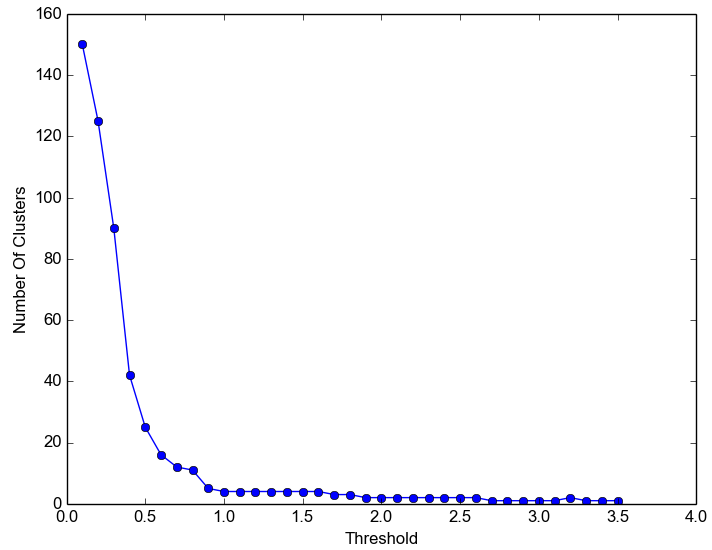
\includegraphics[width=\columnwidth]{figure_1.png}
\caption{Irises Clusters: Number of clusters vary with respect to the value of threshold}
\end{figure}
Then we apply the clustering algorithm on the color pixel dataset. The dataset consists of 150 3-dimensional vectors .
We run the algorithm for the value of threshold $T$ from 1 to half of max euclidean distance of points. The plateau of number of clusters occurs for $K=3$.
\begin{figure}[H]
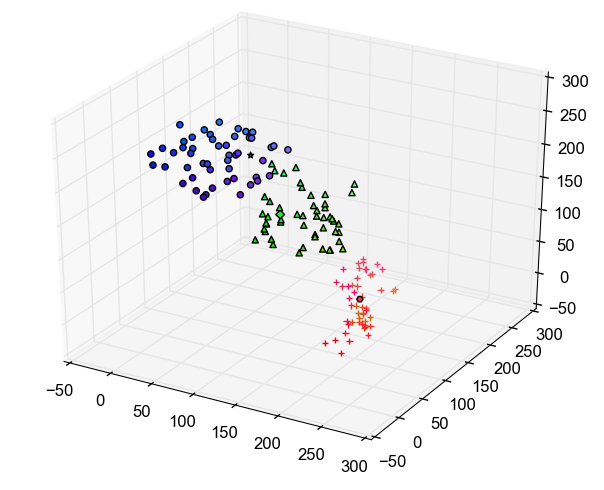
\includegraphics[width=\columnwidth]{figure_2.png}
\caption{pixel clustering: Pixels are clustered into three different clusters.}
\end{figure}
These examples demonstrate that of interest is not only the separation of the objects into a certain number of classes, but also the way in which small classes join into larger ones. These transformations indicate which of small compact classes of objects are close to each other and allow one to understand the intrinsic structure of empirical data. 


\addtolength{\textheight}{-12cm}   % This command serves to balance the 


\begin{thebibliography}{99}

\bibitem{c1} Leonid B. Litinskii, Dmitry E. Romanov, neural network clustering based on distances between objects, ICANN (Athens, Greece, 2006).
\bibitem{c2} SA TommiKarkkainen , Introduction to partitioning-based clustering
methods with a robust example.	2001
\bibitem{c3} Charu C. Aggarwal, Chandan K. Reddy , Data Clustering: Algorithms and Applications. ISBN:1466558210 9781466558212
\bibitem{c4} A. K. Jain, M. N. Murty, P. J. Flynn , Data clustering: a review.
ACM Computing Surveys (CSUR), Volume 31 Issue 3, Sept. 1999 Pages 264-323 
\bibitem{c5} R.A. Fisher , Iris Data Set , UCI machine Learning Laboratory
\bibitem{c6} Jiawei Han, Micheline Kamber and Jian Pei, Data Mining: Concepts and Techniques (3rd ed), ISBN 9780123814791
 

\end{thebibliography}




\end{document}
